\section{Hardware Platform}
\label{cha:ver:sec:Hardware_Platform}

Aus Kostengründen wurde anstelle des FPGA-internen CAN-Controllers ein externer CAN-Controller verwendet. Und viel besser: Dieser CAN-Controller wurde im Unternehmen entwickelt.  Außerdem wurde das von Xilinx entwickelte Board ZCU106 verwendet, das auf dem Zynq Ultracale + MPSoC basiert. Das enthaltene ZU7EV-Gerät(Zynq Ultracale + MPSoC) integriert ein Quad-Core Arm Cortex-A53 Processing System (PS) und einen Dual-Core Arm Cortex-R5F Echtzeit-Prozessor. Das board verfügt auch über viele programmierbare digitale Komponenten, mit denen wiederum eine Vielzahl von Schaltungen realisiert werden können.Wie bereits erwähnt, ist das FPGA Bestandteil des ZCU106 Boards, das im nächsten Kapitel besprochen wird.

\subsection{Xilinx ZCU106 Evaluation Board}

Dieses Kapitel beschreibt die Xilinx ZCU106 Evaluation Board, insbesondere die Bereiche, die diese Plattform einzigartig machen. Dazu gehören die Zynq Ultrasale + MPSoC Architektur, das Processing System (PS) und die Programmable Logik (PL). Die Peripheriegeräte, die für die Interaktion mit dem CAN-Controller erforderlich sind, werden dabei erwähnt. Genauere Informationen dazu findet man im technischen Referenzhandbuch [\cite{XilinxInc.2019}] des Zynq-Plattforms. 

\begin{figure}[h]
	\begin{center}
		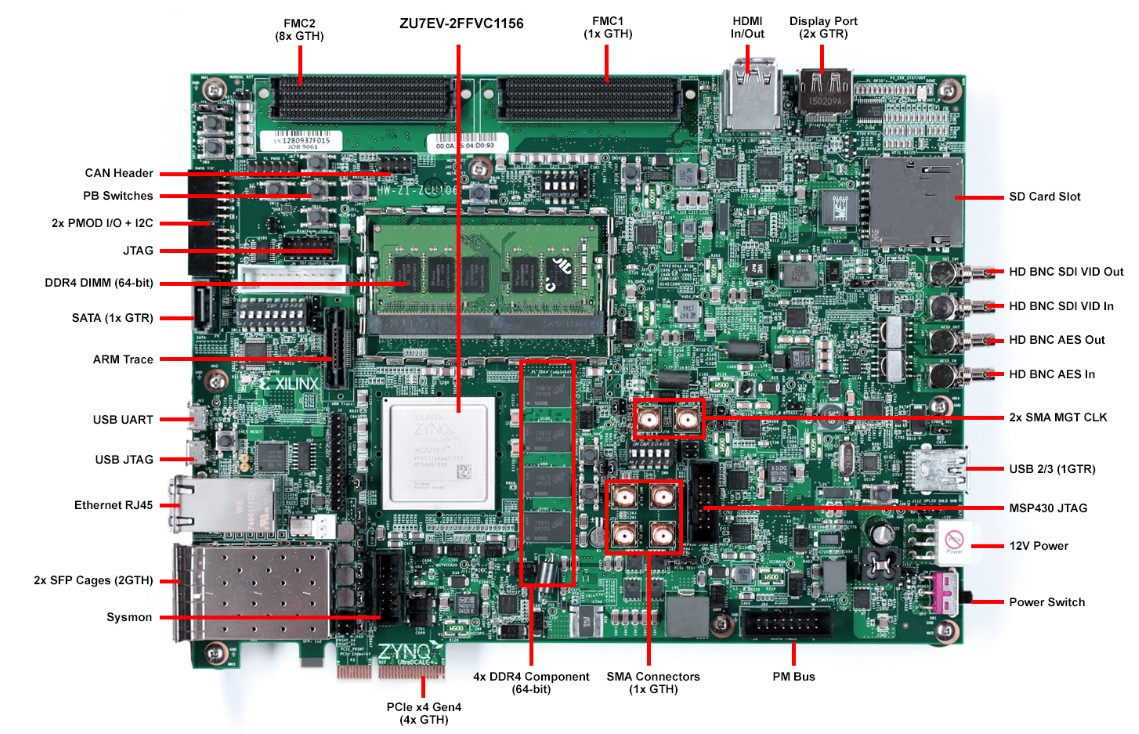
\includegraphics[width=1\textwidth]{./images/zcu106.jpg}
	\end{center}
	\vspace{-5pt}
	\caption[Xilinx ZCU102 Evaluation Board]{Xilinx ZCU102 Evaluation Board [\cite{zcuboard.}]}  %Eckige Klammer (optional): Caption-Text in Abbildungsverzeichnis
	\label{fig:zcu:board}
	\vspace{-5pt}
\end{figure}

%Es ist vorzusehen, dass das Betriebssystem auf mindestens einem der vier physischen Cortex-A53-Prozessoren des ZCU106 laufen wird, mit der Möglichkeit, Bar-Metal-Anwendungen auf anderen Prozessoren laufen zu lassen. 

%\begin{figure}[h]
%	\begin{center}
%		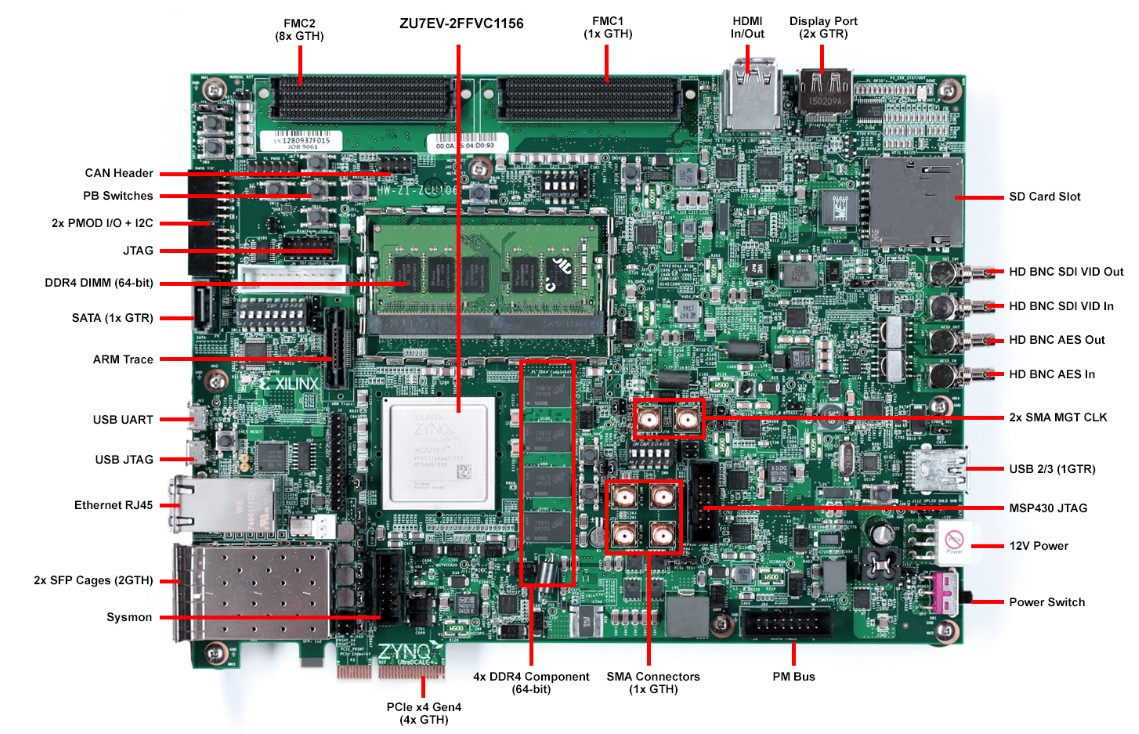
\includegraphics[width=0.98\textwidth]{./images/zcu106.jpg}
%	\end{center}
%	\vspace{-5pt}
%	\caption[Zynq UltraScale+ XCZU7EV-2FFVC1156 MPSoC]{Vortellung des Zynq UltraScale+ XCZU7EV-2FFVC1156 MPSoC} % Eckige Klammer (optional): Caption-Text in Abbildungsverzeichnis
%	\label{fig:zcu106}
%	\vspace{-5pt}
%\end{figure}

\subsubsection{Ultrasale + MPSoC Architektur}
Lassen wir uns, bevor wir uns mit der Zynq Ultrascale+ MPSoC-Architektur beschäftigen, ein wenig über die Zynq-Architektur im Allgemeinen sprechen. Es handelt sich bei Zynq um eine neue Generation von System-on-Chip (SoC), die eine CPU mit einem programmierbaren Logik-FPGA auf demselben Chip kombiniert.
FPGAs sind für ihre besondere Flexibilität beim Entwurf digitaler Schaltungen bekannt. Dennoch ist für viele Anwendungen der Entwurf einer riesigen Zustandsmaschine in Very High Speed Hardware Description Language (VHDL) oder Verilog nicht ausreichend. Stattdessen ziehen wir eine softwareprogrammierbare CPU-Architektur vor, die mit einfacheren FPGA-Blöcken zusammenarbeitet. Im Grunde genommen kann eine CPU jeden Algorithmus ausführen, so lange genug Speicher für ihre Bedürfnisse vorhanden ist. Softwarecode kann schnell geändert, neu kompiliert, gepatcht und debuggt werden. Die Rechenkapazität eines CPU-Kerns allein reicht jedoch oft nicht aus, um eine große Datenmenge zu verarbeiten. weshalb tendieren wir zu parallelen Architekturen, wie Multicore-CPUs, FPGAs und GPUs, um den Rechendurchsatz zu erhöhen.\\

Bislang gab es für jemanden, der eine CPU in Kombination mit einem FPGA benötigte, zwei Möglichkeiten: eine diskrete CPU und ein diskretes FPGA, die über einen Bus miteinander kommunizieren (was zu Bandbreitenbeschränkungen führte), oder eine Soft-Core-CPU. Diese wird direkt in den FPGA programmiert (z.B. 32-Bit Microblaze, 64-Bit Ultrascale, usw.). Die Entscheidung hängt von den Einschränkungen und Anforderungen der Anwendung ab, wie z. B. dem Systempreis, dem Stromverbrauch, der Komplexität und selbstverständlich der Leistung. Xilinx bietet mit der Zynq-Serie ein höheres Maß an Integration mit einer System-on-Chip-Hardcore-ARM-CPU, einem Xilinx-FPGA und Bussen für den effizienten Datentransfer zwischen beiden. Darüber hinaus umfassen die Zynq-Bausteine verschiedene Arten von Input/Output (I/O)-Controllern, Speicherschnittstellen und Hochgeschwindigkeits-Transceivern

\begin{figure}[h]
	\begin{center}
		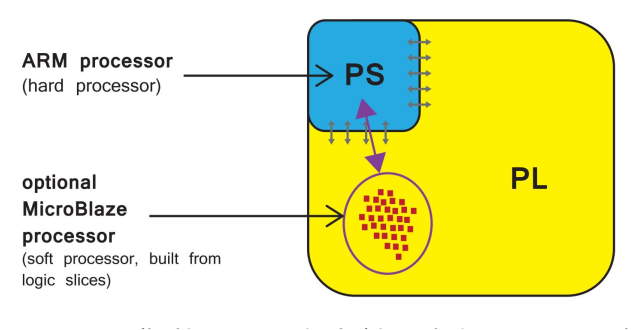
\includegraphics[width=1\textwidth]{./images/ps-pl.jpg}
	\end{center}
	\vspace{-5pt}
	\caption[Hard-(ARM Cortex-A9/Cortex-A53) und Soft-Prozessoren (MicroBlaze)]{Die Anordnung von Hard- (ARM Cortex-A9/Cortex-A53) und Soft-Prozessoren (MicroBlaze) auf einem Zynq/ZynqMP-Baustein [\cite{Crockett:2001018}]}  %Eckige Klammer (optional): Caption-Text in Abbildungsverzeichnis
	\label{fig:pl:ps}
	\vspace{-5pt}
\end{figure}


Die Abbildung ~\ref{fig:pl:ps} zeigt die Trennung zwischen dem festen Logik-Hardware-Prozessor und der programmierbaren Logik, die einen oder mehrere Soft-Prozessoren enthalten kann. 

\subsubsection{Allgemeine Ansicht des Zynq Ultrasale+ MPSoC}
Die Zynq Ultrascale+ MPSoC-Serie ist eine im Jahr 2015 von Xilinx eingeführte moderne SoC-Architektur [\cite{CNXSoftware}]. Abbildung ~\ref{fig:zynqmp:block:diagram} zeigt das Blockdiagramm des Zynq Ultrascale+ EG, der verfügt über mehrere Verarbeitungseinheiten wie die ARM Cortex A53 Application Processing Unit (APU) mit 4 Kernen, die Real-Time Processing Unit (RPU) und die Platform Management Unit (PMU). Die Abbildung zeigt die Schnittstelle zwischen dem Verarbeitungssystem (PS) und der programmierbaren Logik (PL). Die PL verfügt über mehrere Blöcke wie GPIO, Block-RAM und High-Connectivity-Block für die Implementierung von Designs zur Kommunikation mit Peripheriegeräten wie Ethernet oder SPI

\begin{figure}[h]
	\begin{center}
		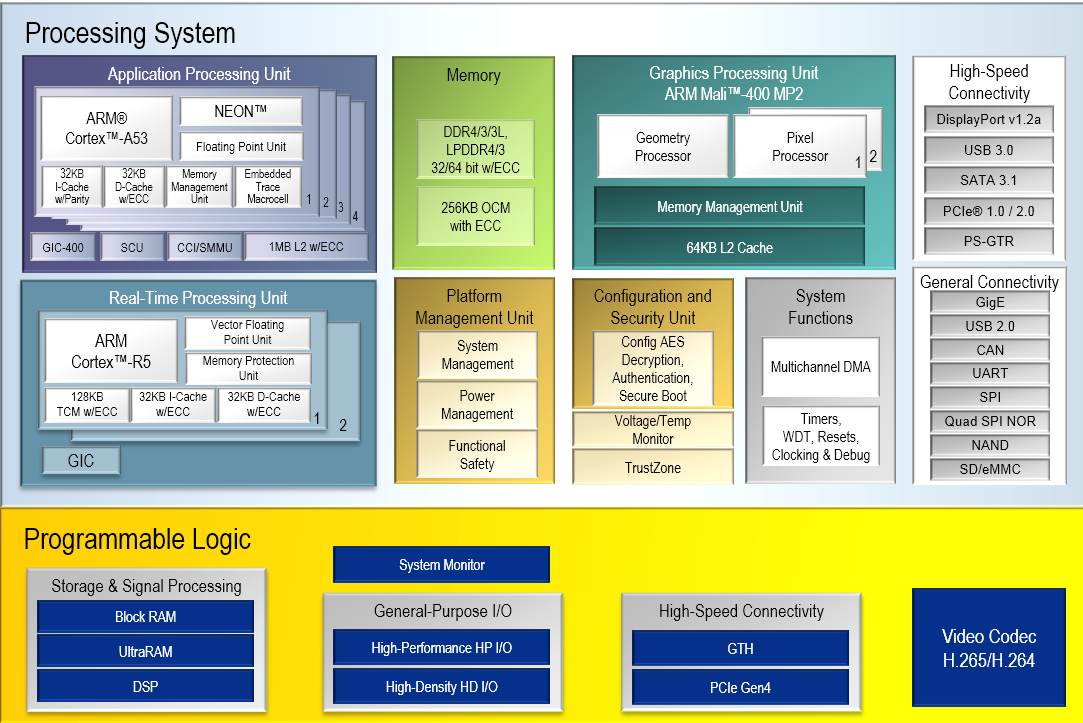
\includegraphics[width=1\textwidth]{./images/zynqmp-blockdiagramm.jpg}
	\end{center}
	\vspace{-5pt}
	\caption[Zynq UltraScale+ MPSoC EV Block Diagram]{Zynq UltraScale+ MPSoC EV Block Diagram [\cite{XilinxInc.}]} % Eckige Klammer (optional): Caption-Text in Abbildungsverzeichnis
	\label{fig:zynqmp:block:diagram}
	\vspace{-5pt}
\end{figure}

 Im Folgenden findet sich eine Liste der besonderen Komponente dieser Familie:
 \begin{itemize}
 	\item \textbf{APU}
 	\begin{itemize}
 		\item 64-bit Quad-core ARM Cortex-A53 1.5 GHz
 		\item NEON Media Processing Engine + Floating Point Unit (FPU)
 		\item Unterstützung für 32/64-Bit-Betriebsmodi
 		\item 32 KB Level-1 cache
 		\item 1 MB Level-2 cache
 	\end{itemize}
 	\item \textbf{RPU}
 	\begin{itemize}
 		\item 32-bit Dual-core ARM Cortex-R5  600 MHz
 	\end{itemize}
 	\item \textbf{graphics processing uni(GPU)}
 	\begin{itemize}
 		\item ARM Mali-400 MP2
 	\end{itemize}
 	\item \textbf{On-Chip Memory (OCM)}: 256KB
 	\item \textbf{Zwei 8-Channel Direct Memory Access (DMA) controllers}
 	\item \textbf{System Memory Management Unit (SMMU)}
 	\item \textbf{Platform Management Unit (PMU)}
 \end{itemize}
 
Der PS unterstützt auch viele Eingangs-/Ausgangsschnittstellen wie SRAM-Schnittstellen (SD, QSPI, NAND), GPIOs, UART usw.

\begin{figure}[h]
	\begin{center}
		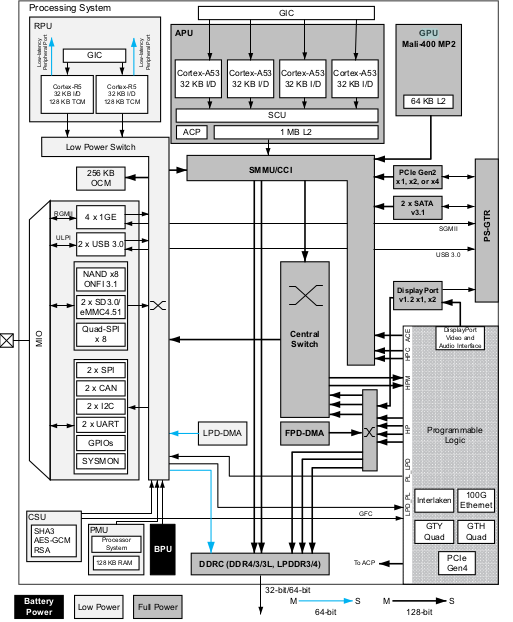
\includegraphics[width=1\textwidth]{./images/top-level_zynqmp.jpg}
	\end{center}
	\vspace{-5pt}
	\caption[Zynq UltraScale+ MPSoC Top-Level Blockdiagramm]{Zynq UltraScale+ MPSoC Top-Level Blockdiagramm [\cite{XilinxInc.2019}]} % Eckige Klammer (optional): Caption-Text in Abbildungsverzeichnis
	\label{fig:zynqmp:top:level}
	\vspace{-5pt}
\end{figure}
Im Top-Level-Blockdiagramm der Zynq MPSoC-Architektur ~\ref{fig:zynqmp:top:level} ist die Verbindung zwischen den verschiedenen Blöcken markiert. Da kann die verschiedenen Verarbeitungseinheiten (APU, RPU, GPU) sowie viele Verbindungen zwischen den Blöcken finden. Zu beachten ist, dass die Richtung der Pfeile die Prioritätsreihenfolge zwischen Master und Slave festlegt.
Sie haben vielleicht bemerkt, dass in Abbildung ~\ref{fig:zynqmp:block:diagram} erwähnt wird, dass es sich um das Blockdiagramm für die EV-Variante handelt. Tatsächlich gibt es drei Varianten des Zynq MPSoC, die wie folgt gekennzeichnet sind:

\begin{itemize}
	\item \textbf{CG}: Mittelklasse-Gerät, mit Dual Cortex-A53 und Dual Cortex-R5.
	\item \textbf{EG}: High-End-Gerät, mit Quad-Cortex-A53, Dual-Core-Cortex-R5 und Mali-GPU
	\item \textbf{EV}: High-End-Gerät, mit Quad Cortex-A53, Dual-Core Cortex-R5, Mali GPU und Video-Codec (H.264, H.265).
\end{itemize}

Die beiden Hauptkomponenten des ZynqMP, das Verarbeitungssystem und die programmierbare Logik, werden im Folgenden ausführlicher beschrieben.

\subsubsection{Processing System (PS)}
Das ZynqMP-Verarbeitungssystem umfasst einerseits den ARM-Prozessor, anderseits aber auch mehrere zugehörige Verarbeitungsmodule, die eine Application Processing Unit (APU) bilden, sowie weitere Schnittstellen für Peripheriegeräte, Cache-Speicher, Speicherschnittstellen, Verbindungs- und Takterzeugungsschaltungen. Die APU besteht aus einem speziellen ARM Cortex-A53 MPCore (Quad oder Dual). In der ARM-Gerätefamilie gelten diese als relativ stromsparend, sind aber in der Lage, ein vollwertiges Betriebssystem wie Linux, Android oder ähnliches auszuführen

\begin{figure}[h]
	\begin{center}
		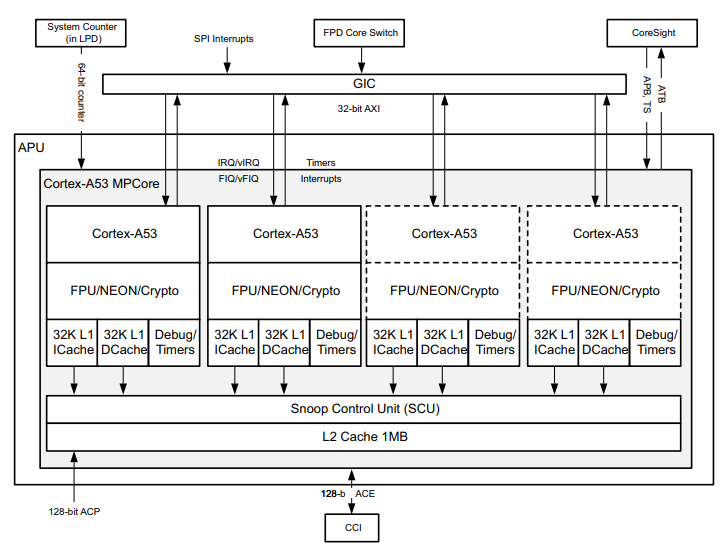
\includegraphics[width=1\textwidth]{./images/apu.jpg}
	\end{center}
	\vspace{-5pt}
	\caption[Detailliertes APU-Blockdiagramm]{Detailliertes APU-Blockdiagramm [\cite{Xilinx2017}[p.~57]]} % Eckige Klammer (optional): Caption-Text in Abbildungsverzeichnis
	\label{fig:zynqmp:apu}
	\vspace{-5pt}
\end{figure}

Abbildung ~\ref{fig:zynqmp:apu} fasst einige wichtige Merkmale der APU zusammen. So verfügt sie beispielsweise über einen separaten 32-KB-Cache der Ebene 1 für Befehle und Daten und einen gemeinsamen 1-MB-Cache der Ebene 2. Eine Snoop Control Unit (SCU) sorgt für Cache-Kohärenz zwischen den Kernen und zeigt an, wenn die Daten ungültig sind.\\
Der L2-Cache-Controller APU kommuniziert mit dem Rest des SoC über eine 128-Bit AXI Coherency Extension (ACE) Master-Schnittstelle zur Cache Coherent Interconnect\\
Andererseits kann ein 128-Bit-Accelerator Coherency Port (ACP) Slave-Controller verwendet werden, wenn ein anderer Block mit Master-Zugriff auf Daten im L2-Cache zugreifen möchte. In der Praxis bedeutet dies, dass der PL auf den L2-Cache über den Port S_AXI_ACP_FPD zugriffen kann.

\subsubsection{Programmable Logik (PL)}
Dieser Abschnitt bietet einen Überblick über die verfügbaren Funktionen der Zynq Ultrascale+ MPSoC Programmable Logic (PL). Tabelle ~\ref{tab:zcu:vergleich} ist ein Vergleich einiger EG-Bausteine. Es gibt tatsächlich mehr Varianten als die dort aufgeführten. Die FPGA-Fabric besteht hauptsächlich aus Logikzellen und konfigurierbaren Logikblöcken (CLB). Ein CLB kann Flipflops und eine Look-up-Table (LUT) enthalten, muss es aber nicht.\\

\begin{table}[htbp]
	\centering
	\begin{tabular}{|p{5cm}|p{2cm}|p{2cm}|p{2cm}|}
		\toprule
		\textbf{Gerät Name} & ZU4EV & ZU5EV & ZU7EV \\
		\midrule
		\textbf{System Logic Cells (K)} & 192 & 256 & 504 \\
		\textbf{Speicher (Mb)} & 18.5 & 23.1 & 38.0 \\
		\textbf{DSP-Schnitte} & 728 & 1,248 & 1,728 \\
		\textbf{Video-Code-Einheit (VCU)} & 1 & 1 & 1 \\
		\textbf{Maximale E/A-Pins} & 252 & 252 & 464 \\
		\bottomrule
	\end{tabular}
	\caption[Vergleich einiger Zynq Ultrascale+ MPSoC EG ]{Vergleich einiger Zynq Ultrascale+ MPSoC EG [\cite{XilinxInc.}]}
	\label{tab:zcu:vergleich}
\end{table}

Der Speicher eines FPGAs besteht entweder aus dedizierten Speicherblöcken wie BlockRAM und UltraRAM oder aus CLB, die als RAM-Zellen verwendet werden (Distributed RAM). Schließlich enthält das FPGA eine Reihe von DSP48E2 IP-Blöcken, die Multiplikationen und andere arithmetische/logische Aufgaben effizient durchführen können

\subsection{MCP251XFD CAN Controller + Transceiver}
Bevor wir uns näher mit diesem CAN-Controller befassen, sollte erklärt werden, dass das \grqq x\grqq\ im Namen des Chips entweder \grqq 7\grqq\ oder \grqq 8\grqq\ werden kann. MCP251XFD unterstützt also MCP2517FD und MCP2518FD.\\
Die Firma entwickelte im Rahmen dieses Projekt, aus kostengünstigen Gründen den  MCP2517FD. Zweck war es, zu prüfen, wie schnell Daten mit diesem CAN-Controller verarbeitet werden können. Auf die Eigenschaften des Chips wird nun im Folgenden eingegangen.

\begin{figure}[h]
	\begin{center}
		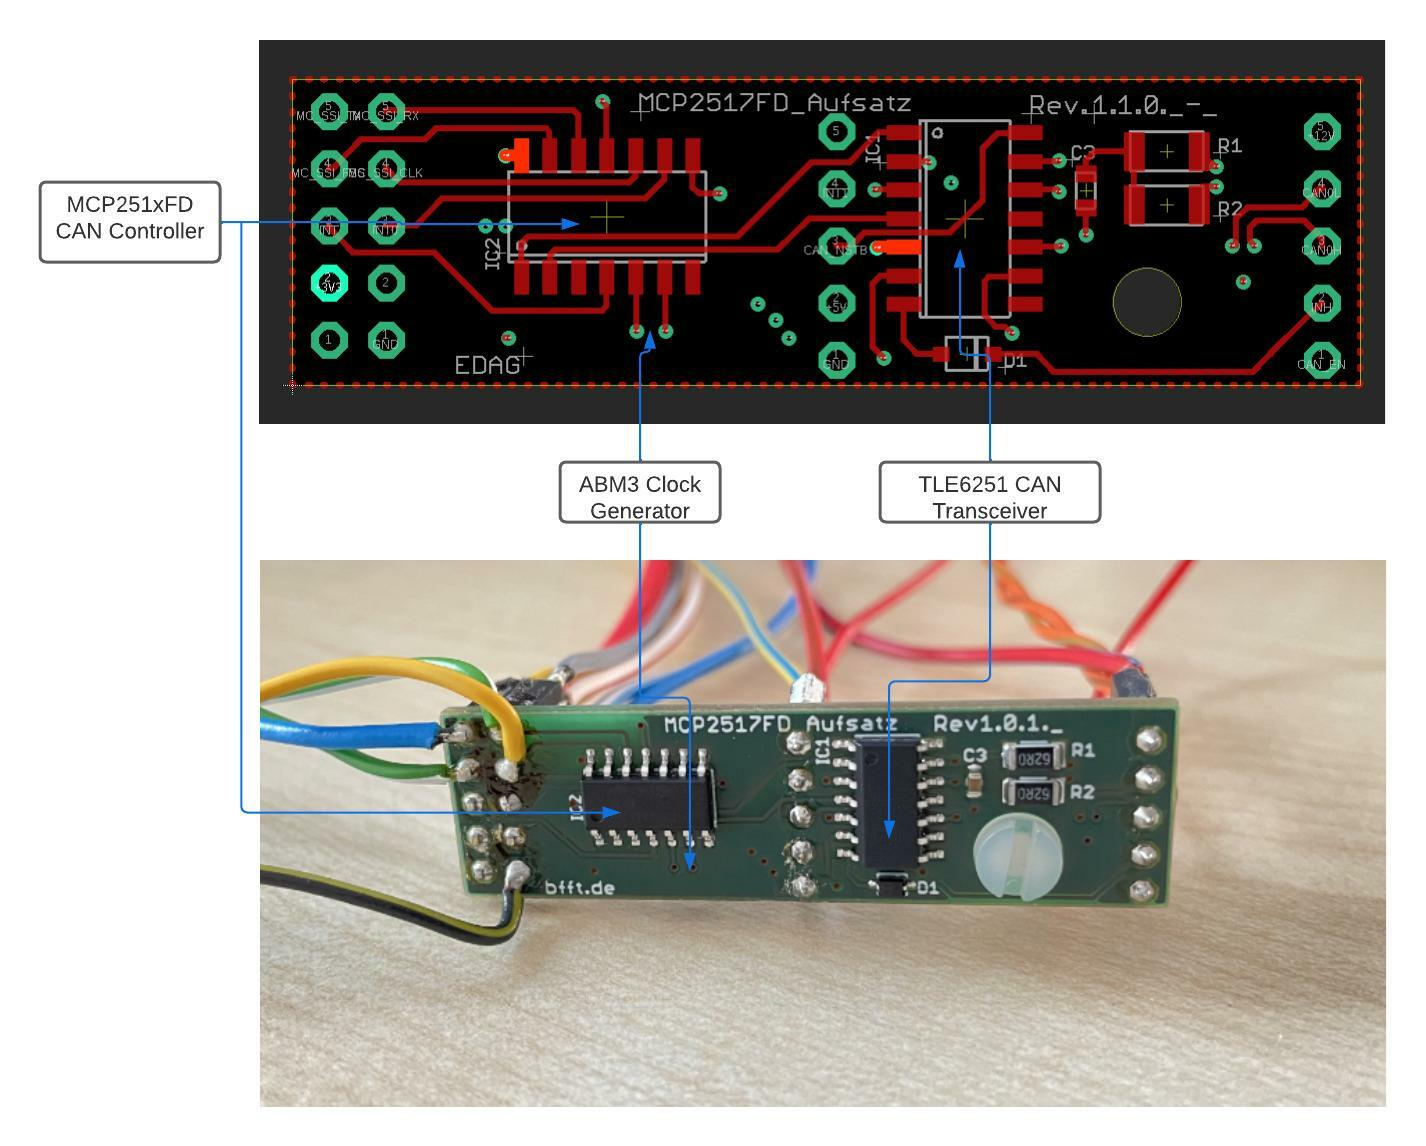
\includegraphics[width=1\textwidth]{./images/mcp_ic_phy.jpg}
	\end{center}
	\vspace{-5pt}
	\caption[CAN-Transceiver- und Controller-Modul]{CAN-Transceiver- und Controller-Modul} % Eckige Klammer (optional): Caption-Text in Abbildungsverzeichnis
	\label{fig:can:controller:transciever}
	\vspace{-5pt}
\end{figure}

Der MCP2517FD-Chip ist ein kompaktes Board, das eine komplette CAN-Lösung bietet und als Steuerknoten in einem CAN-Netzwerk verwendet wird. Wie in Abbildung 1 zu sehen ist, besteht das Board hauptsächlich aus einem CAN-FD-Controller mit SPI-Schnittstelle (MCP2517FD) und einem Hochgeschwindigkeits-CAN-Transceiver (TLE6251). Letzterer stellt eine physikalische Verbindung mit dem CAN-Bus selbst her, während der CAN-Controller MCP2517FD eine Schnittstelle zwischen der MCU und dem PHY darstellt. Die Aufgabe des CAN-Controllers seinerseits ist es, die Arbitrierung, das Nachrichtenframing, die Nachrichtenvalidierung, die Fehlererkennung, die Nachrichtenfilterung und vieles mehr zu übernehmen. Weiterhin unterstützt er sowohl CAN-Frames im klassischen Format (CAN2.0B) als auch im CAN-Flexible-Data-Rate-Format (CAN FD), wie in ISO 11898- 1:2015.\\
Der ISO 11898- 1:2015 hier, der von der International Organization for Standardization (ISO) rausgegeben wurde, spezifiziert das klassische CAN-Rahmenformat und das neu eingeführte CAN Flexible Data Rate Frame Format. Das klassische CAN-Frame-Format erlaubt Bitraten bis zu 1 Mbit/s und Nutzdaten bis zu 8 Byte pro Frame, Das Flexible Data Rate Frame Format erlaubt höhere Bitraten als 1 Mbit/s und Nutzdaten von mehr als 8 Byte pro Frame.

\subsubsection{CAN FD Controller Modul}

\begin{figure}[h]
	\begin{center}
		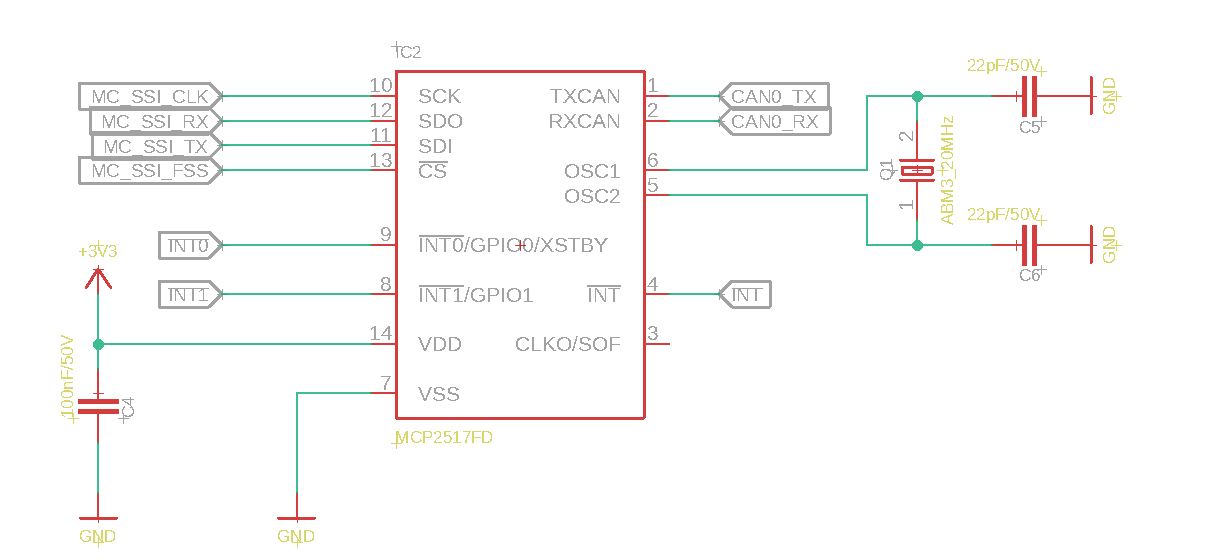
\includegraphics[width=1\textwidth]{./images/mcp_eagle.jpg}
	\end{center}
	\vspace{-5pt}
	\caption[CAN Controller Modul]{CAN Controller Modul} % Eckige Klammer (optional): Caption-Text in Abbildungsverzeichnis
	\label{fig:can:controller}
	\vspace{-5pt}
\end{figure}

Der MCP2517FD enthält die folgenden Hauptblöcke[\cite{Transmission2018}]:
\begin{itemize}
	\item Das CAN FD Controller-Modul implementiert das CAN FD-Protokoll und enthält die FIFOs und Filter.
	\item Die SPI-Schnittstelle, die zur Steuerung des Geräts durch Zugriff auf SFRs und RAM verwendet wird
	\item Der RAM-Controller arbitriert die RAM-Zugriffe zwischen dem SPI- und dem CAN FD Controller-Modul
	\item Der Nachrichten-RAM, der zur Speicherung der Daten der Nachrichtenobjekte verwendet wird
	\item Der Oszillator: Das MCP251XFD CAN Controller verwendet den ABM3 Clock Generator, als Standardtaktquelle für den Chip. Der ABM3 auf diesem Board wurde so programmiert, dass er eine Ausgangsfrequenz von 20 MHz erzeugt.
	
\end{itemize}

Der Controller kann in verschiedenen Modi eingestellt werden, nämlich
\begin{itemize}
	\item Configuration
	\item Normal CAN FD
	\item Normal CAN 2.0
	\item Sleep
	\item Listen Only
	\item Restricted Operation: Also Eingeschränkter Betrieb
	\item und Internal and External Loop back modes (Interner und externer Loopback-Modus)
\end{itemize}
\subsubsection{TLE6251 CAN Transceiver}

\begin{figure}[h]
	\begin{center}
		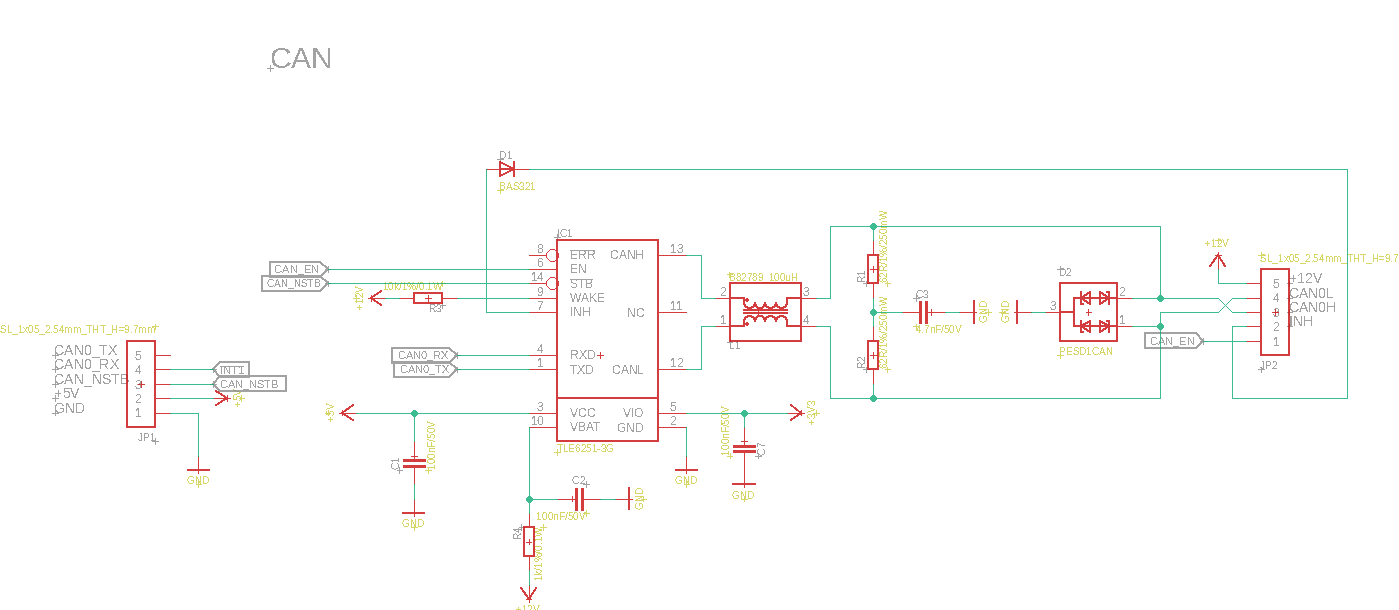
\includegraphics[width=1.2\textwidth]{./images/can_transceiver_eagle.jpg}
	\end{center}
	\vspace{-5pt}
	\caption[CAN Transceiver Modul]{CAN Transceiver Modul} % Eckige Klammer (optional): Caption-Text in Abbildungsverzeichnis
	\label{fig:can:transceiver}
	\vspace{-5pt}
\end{figure}

Der Hochgeschwindigkeits-CAN-Transceiver, der TLE6251, stellt eine physische Verbindung mit dem CAN-Bus her. Dieser ermöglicht eine Kommunikationsgeschwindigkeit von bis zu 5Mbps und unterstützt die Betriebsmodi Normal und Standby. Der Normalmodus ist eingeschaltet, wenn der STBY-Pin, der auf den AN-Pin der mikroBUS geführt wird, auf einem logischen Low-Pegel liegt, während der TXD-Pin auf einem hohen logischen Pegel gehalten wird. Im Normalmodus können die Daten über die CAN H/L-Busleitungen gesendet und empfangen werden.


